%Problem Set 1
%%%%%%%%%%%%%%%%%%%%%%%%%%%%%%%%%%%%%%%%%%%%%%%%

%Sweave('C:/Klaus/AAEC5126/problemsets/ps1',syntax=SweaveSyntaxNoweb)

%I) DEFINE DOCUMENTCLASS AND LOAD ALL REQUIRED PACKAGES

\documentclass[11pt,reqno]{article}   %keep it simple
\usepackage{hyperref}
\usepackage{graphicx}      % for fancy graphics
\usepackage{setspace}      % for basic formatting
\usepackage{enumerate} 
\usepackage[fleqn]{amsmath}
\usepackage{enumitem}% for more flexibility with numbered lists
  %KEY - this preserves R formatting and comments

% You may need to load all or some of these packages -
%follow the instructions on our course web site under "Help with LaTex"

%II) PREAMBLE
%%%%%%%%%%%%%%%%%%%%%%%%%%%%%%%%%%%%%%%%%%%%%%%%%%
\pagestyle{plain} %puts page number center bottom
\setlength{\topmargin}{0in}
\setlength{\textheight}{8.5in}
\setlength{\oddsidemargin}{.0in}
\setlength{\evensidemargin}{.0in}
\setlength{\textwidth}{6.5in}
\setlength{\footskip}{.5in}
\setlength{\parindent}{0in} %suppress indentation
%\onehalfspacing

\newcommand{\mlt}[1]{\mathbf{#1}} %matrix bold for Latin symbols
\newcommand{\mgr}[1]{\boldsymbol{#1}}%matrix bold for Greek symbols
\newcommand{\kR}{\tt R\rm{} }%shortcut for "R" symbol
\newcommand{\ksp}{\vspace{0.1in}}   % insert some space between chunks
%feel free to add your own shortcuts  - here a mine:
\newcommand{\kl}{\left(}
\newcommand{\kr}{\right)}
\newcommand{\kll}{\left\{}
\newcommand{\krr}{\right\}}
\newcommand{\kmu}{\mgr{\mu}}
\newcommand{\kpsi}{\mgr{\psi}}
\newcommand{\kphi}{\mgr{\phi}}
\newcommand{\kgam}{\mgr{\gamma}}
\newcommand{\ktheta}{\mgr{\theta}}
\newcommand{\kbeta}{\mgr{\beta}}
\newcommand{\kdelta}{\mgr{\delta}}
\newcommand{\kt}{^{\prime}}
\newcommand{\kdel}{\partial}
\newcommand{\kdot}{\kl . \kr}
\newcommand{\keps}{\epsilon}
\newcommand{\kx}{\mlt{x}}
\newcommand{\kX}{\mlt{X}}
\newcommand{\kV}{\mlt{V}}
\newcommand{\kM}{\mlt{M}}
\newcommand{\kP}{\mlt{P}}
\newcommand{\ky}{\mlt{y}}
\newcommand{\kb}{\mlt{b}}
\newcommand{\ki}{\mlt{i}}
\newcommand{\ke}{\mlt{e}}
\newcommand{\klam}{\lambda}
\newcommand{\kp}{\mlt{p}}
\newcommand{\kprob}{\text{prob}}
\newcommand{\kz}{\mlt{z}}
\newcommand{\ksig}{\sigma^2}
\newcommand{\kSig}{\mgr{\Sigma}}
\newcommand{\klog}{\text{log}}
\newcommand{\kols}{\kl \kX\kt\kX\kr^{-1}\kX\kt\ky}
\newcommand{\kSSE}{\kl \ky-\kX\kb\kr\kt\kl\ky-\kX\kb\kr}

\setlist{nolistsep,leftmargin=*} %tighter bullets - requires package enumitem

%%%%%%%%%%%%%%%%%%%%%%%%
\usepackage{Sweave}
\begin{document}
\Sconcordance{concordance:ps1.tex:ps1.rnw:%
1 73 1 1 0 10 1 1 12 11 1 1 2 1 0 6 1 3 0 1 2 3 1 1 2 %
5 0 1 2 6 1 1 8 10 0 1 2 1 3 12 0 1 2 2 1 1 2 1 0 3 1 %
3 0 1 2 2 1 1 2 1 0 7 1 3 0 1 2 1 7 6 0 1 1 3 0 1 4 %
13 0 1 4 10 1 1 2 1 0 1 1 3 0 1 2 2 1 1 2 1 0 6 1 3 0 %
1 3 1 0 1 6 5 0 1 1 3 0 1 2 1 3 12 0 1 4 18 1 1 2 1 0 %
4 1 3 0 1 2 3 1 1 2 5 0 1 2 1 8 10 0 1 2 1 3 12 0 1 2 %
2 1 1 2 1 0 3 1 1 2 6 1 3 0 1 2 1 7 6 0 1 1 3 0 1 2 1 %
3 13 0 1 4 5 1 1 2 1 0 9 1 3 0 1 2 2 1 1 7 6 0 1 1 3 %
0 1 2 1 3 12 0 1 4 23 1 1 3 2 0 1 3 2 0 1 1 3 0 1 2 1 %
4 6 0 1 2 1 3 16 0 1 2 5 1 1 2 1 0 1 1 3 0 1 2 1 3 15 %
0 1 2 1 8 1 3 3 1 1 2 1 0 5 1 1 2 6 1 3 0 1 2 1 6 5 0 %
1 1 3 0 1 2 1 3 16 0 1 2 11 1 1 2 1 0 5 1 1 2 6 1 3 0 %
1 2 1 6 5 0 1 1 3 0 1 2 1 3 15 0 1 2 54 1 1 2 8 0 1 2 %
2 1}

%%%%%%%%%%%%%%%%%%%%%%%%

%III) TOP MATTER INFORMATION
\title{Problem Set 1}
\author{Nima Mohammadi \\ \href{mailto:nimamo@vt.edu}{\textbf{nimamo@vt.edu}}} %ENTER YOUR NAME HERE

\maketitle %this comes at the end of the top matter to set it.

%Set basic R-options upfront and load all required R packages:

%%%%%%%%%%%%%%%%%%%%%%%%%%%%%%%%%%%%%%%%%%%%%%%%%%%%%%%%%%%%%%%%%%%%%%%%
\section*{Question 1: Omitting regressors under independence and dependence}
%%%%%%%%%%%%%%%%%%%%%%%%%%%%%%%%%%%%%%%%%%%%%%%%%%%%%%%%%%%%%%%%%%%%%%%%%%

\textbf{Part A: Independence, Full Model}
%%%%%%%%%%%%%%%%%%%%%%%%%%%%%%%%%%%%%%%%%%%
\begin{enumerate}
\item
Generate two independent, normally distributed regressors (= explanatory variables), one with mean 2 and std 1,
the other with mean 3 and std 1.  Set the sample size to 1000 observations in each case. Call these variables
x1 and x2
\begin{Schunk}
\begin{Sinput}
R> n <- 1000
R> x1mean <- 2
R> x1std <- 1
R> x1 <- matrix(rnorm(n, x1mean, x1std), n)
R> x2mean <- 3
R> x2std <- 1
R> x2 <- matrix(rnorm(n, x2mean, x2std), n)
\end{Sinput}
\end{Schunk}
\newpage
\item Create a scatterplot to examine the relationship between x1 and x2.
\begin{figure}[!ht]
\centering
\begin{Schunk}
\begin{Sinput}
R> plot(x1, x2)
\end{Sinput}
\end{Schunk}
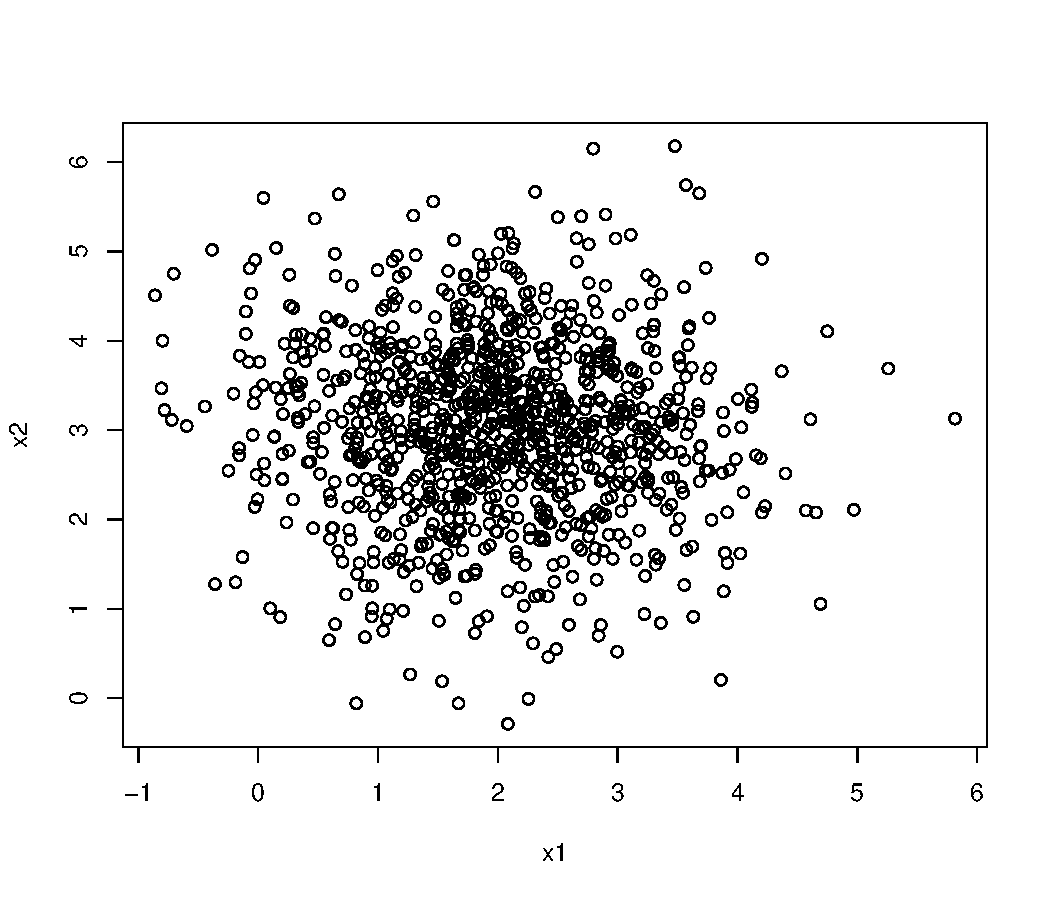
\includegraphics{ps1-chunk1-2}

\caption{Scatterplot of x1 and x2}
\label{fig:scatter}
\end{figure}

\item Create a table of sample statistics, including the correlation coefficient

\begin{Schunk}
\begin{Sinput}
R> df <- data.frame("var"=c("$x_1$", "$x_2$"),
+                  "mean"=c(mean(x1), mean(x2)),
+                  "std"=c(sd(x1), sd(x2)),
+                  "min"=c(min(x1), min(x2)),
+                  "max"=c(max(x1), max(x2)),
+                  "correlation"=c(cor(x1, x2), cor(x1, x2))
+                  )
\end{Sinput}
\end{Schunk}

% latex table generated in R 3.6.2 by xtable 1.8-4 package
% Tue Feb 11 02:13:28 2020
\begin{table}[!h]
\centering
\caption{Sample statistics for $x_1$ and $x_2$} 
\begin{tabular}{lrrrrr}
  \hline
var & mean & std & min & max & correlation \\ 
  \hline
$x_1$ & 1.9816 & 1.0166 & -0.8613 & 5.8147 & -0.0460 \\ 
  $x_2$ & 3.0349 & 1.0174 & -0.2876 & 6.1790 & -0.0460 \\ 
   \hline
\end{tabular}
\end{table}
\item Draw a normal(0,1) error term, define a vector of true parameters for the constant, x1, and x2 of
$\left[1,1,-1\right]$, and build your dependent variable.
\begin{Schunk}
\begin{Sinput}
R> eps <- rnorm(n)
R> X <- cbind(rep(1, n), x1, x2)
R> bvec <- c(1, 1, -1)
R> y <- X %*% bvec + eps
\end{Sinput}
\end{Schunk}

\item Run an OLS regression on the full model. Show the output table. Call this model "Independent, full"

\begin{Schunk}
\begin{Sinput}
R> bols <- solve(t(X) %*% X) %*% (t(X) %*% y)
R> e <- y - X %*% bols
R> k <- ncol(X)
R> s2 <- (t(e) %*% e) / (n-k)
R> Vb <- s2[1, 1] * solve(t(X) %*% X)
R> se <- sqrt(diag(Vb))
R> t <- bols / se
R> SSRindep <- t(e) %*% e
\end{Sinput}
\end{Schunk}

\begin{Schunk}
\begin{Sinput}
R> df2 <- data.frame(col1=c("constant", "$x_1$", "$x_2$"),
+                  col2=bvec,
+                  col3=bols,
+                  col4=se,
+                  col5=t
+                  )
R> colnames(df2) <- c("variable", "true value", "estimate", "s.e.", "t")
\end{Sinput}
\end{Schunk}
% latex table generated in R 3.6.2 by xtable 1.8-4 package
% Tue Feb 11 02:13:28 2020
\begin{table}[!h]
\centering
\caption{OLS Estimation - Independent, Full} 
\begin{tabular}{lrrrr}
  \hline
variable & true value & estimate & s.e. & t \\ 
  \hline
constant & 1.0000 & 0.8647 & 0.1197 & 7.2242 \\ 
  $x_1$ & 1.0000 & 1.0435 & 0.0312 & 33.4307 \\ 
  $x_2$ & -1.0000 & -0.9794 & 0.0312 & -31.4050 \\ 
   \hline
\end{tabular}
\end{table}\end{enumerate}


\textbf{Part B: Independence, Omitted}
%%%%%%%%%%%%%%%%%%%%%%%%%%%%%%%%%%%%%%%%%%%

\begin{enumerate}
\item
Next, drop the last column in X (your x2).
Update your ``k'' value accordingly.

\begin{Schunk}
\begin{Sinput}
R> X <- X[, -k]
R> k <- ncol(X)
\end{Sinput}
\end{Schunk}

\item
Re-run the regression and capture the output. Call this model "Independent, Omit".
\begin{Schunk}
\begin{Sinput}
R> bols <- solve(t(X) %*% X) %*% (t(X) %*% y)
R> e <- y - X %*% bols
R> s2 <- (t(e) %*% e) / (n-k)
R> Vb <- s2[1, 1] * solve(t(X) %*% X)
R> se <- sqrt(diag(Vb))
R> t <- bols / se
R> SSRindepOmit <- t(e) %*% e
\end{Sinput}
\end{Schunk}
\begin{Schunk}
\begin{Sinput}
R> bvec <- c(1, 1)
R> df3 <- data.frame(col1=c("constant", "$x_1$"),
+                  col2=bvec,
+                  col3=bols,
+                  col4=se,
+                  col5=t
+                  )
R> colnames(df3) <- c("variable", "true value", "estimate", "s.e.", "t")
\end{Sinput}
\end{Schunk}

% latex table generated in R 3.6.2 by xtable 1.8-4 package
% Tue Feb 11 02:13:28 2020
\begin{table}[!h]
\centering
\caption{OLS Estimation - Independent, Omit} 
\begin{tabular}{lrrrr}
  \hline
variable & true value & estimate & s.e. & t \\ 
  \hline
constant & 1.0000 & -2.1972 & 0.0979 & -22.4474 \\ 
  $x_1$ & 1.0000 & 1.0886 & 0.0440 & 24.7664 \\ 
   \hline
\end{tabular}
\end{table}\item
Comment on the estimated coefficient for x1 (with x2 omitted).
Therefore, what can you conclude regarding the effects of an omitted variable that is independent from all included variables on the remaining coefficients?\\

We can see that by omitting a relevant variable, namely x2, the estimated effects of the included variables change depending on the potential correlation that may exist between those variables and the ommited variable. Whereas the esimated value for coefficient of x1 is still very close to the true value, we can see that it has clearly impacted our estimation of the constant term. This results from the fact that x1 and x2 are independent.
\end{enumerate}


\textbf{Part C: Correlation, full model}\\
%%%%%%%%%%%%%%%%%%%%%%%%%%%%%%%%%%%%%%%%%%%%%%%%%%%%%%%%%%
Continue with you original sweave file - \textbf{do NOT re-set the random number seed!}\\

\begin{enumerate}
\item
Generate two correlated regressors (= explanatory variables), one with mean 2 and std 1, 
the other with mean 3 and std 1, and with covariance (correlation in this case) of 0.8.  
Set the sample size to 1000 as before.  
Use the "mvrnorm" function in the MASS package to obtain the correlated draws (some help with this is given below)

\begin{Schunk}
\begin{Sinput}
R> m <- c(2, 3)
R> V <- matrix(c(1, 0.8, 0.8, 1), nrow=2)
R> X <- mvrnorm(n=n, m, V)
R> x1 <- X[, 1]
R> x2 <- X[, 2]
\end{Sinput}
\end{Schunk}

\item
Generate a scatter plot and a table with sample statistics, including correlation

\begin{Schunk}
\begin{Sinput}
R> plot(x1, x2)
\end{Sinput}
\end{Schunk}
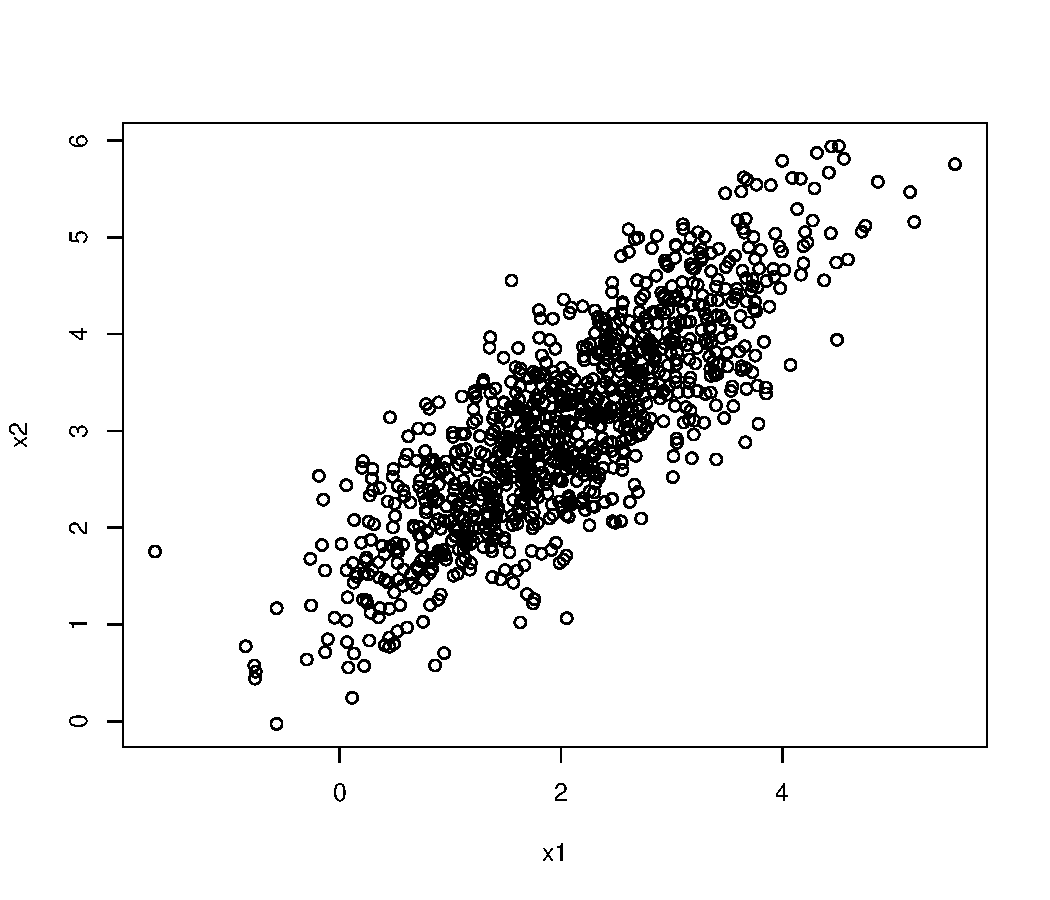
\includegraphics{ps1-chunk3-2}

\begin{Schunk}
\begin{Sinput}
R> df <- data.frame("var"=c("$x_1$", "$x_2$"),
+                  "mean"=c(mean(x1), mean(x2)),
+                  "std"=c(sd(x1), sd(x2)),
+                  "min"=c(min(x1), min(x2)),
+                  "max"=c(max(x1), max(x2)),
+                  "correlation"=c(cor(x1, x2), cor(x1, x2))
+                  )
\end{Sinput}
\end{Schunk}

% latex table generated in R 3.6.2 by xtable 1.8-4 package
% Tue Feb 11 02:13:28 2020
\begin{table}[!h]
\centering
\caption{Sample statistics for $x_1$ and $x_2$} 
\begin{tabular}{lrrrrr}
  \hline
var & mean & std & min & max & correlation \\ 
  \hline
$x_1$ & 2.0495 & 1.0598 & -1.6692 & 5.5605 & 0.8221 \\ 
  $x_2$ & 3.0563 & 1.0516 & -0.0266 & 5.9435 & 0.8221 \\ 
   \hline
\end{tabular}
\end{table}\item
\textbf{Use the same betas and error draws from before} and compute a new $y$ variable.
Run the full model. Call it "Correlated, full". Are there any noteworthy changes compared to the original model ("Independent, full")?
\begin{Schunk}
\begin{Sinput}
R> X <- cbind(rep(1, n), x1, x2)
R> bvec <- c(1, 1, -1)
R> y <- X %*% bvec + eps
R> k <- ncol(X)
R> bols <- solve(t(X) %*% X) %*% (t(X) %*% y)
R> e <- y - X %*% bols
R> s2 <- (t(e) %*% e) / (n-k)
R> Vb <- s2[1, 1] * solve(t(X) %*% X)
R> se <- sqrt(diag(Vb))
R> t <- bols / se
R> SSRcorr <- t(e) %*% e
\end{Sinput}
\end{Schunk}

\begin{Schunk}
\begin{Sinput}
R> df4 <- data.frame(col1=c("constant", "$x_1$", "$x_2$"),
+                  col2=bvec,
+                  col3=bols,
+                  col4=se,
+                  col5=t
+                  )
R> colnames(df4) <- c("variable", "true value", "estimate", "s.e.", "t")
\end{Sinput}
\end{Schunk}

% latex table generated in R 3.6.2 by xtable 1.8-4 package
% Tue Feb 11 02:13:28 2020
\begin{table}[!h]
\centering
\caption{OLS Estimation - Correlated, Full} 
\begin{tabular}{lrrrr}
  \hline
variable & true value & estimate & s.e. & t \\ 
  \hline
constant & 1.0000 & 0.7641 & 0.1004 & 7.6099 \\ 
  $x_1$ & 1.0000 & 0.9343 & 0.0524 & 17.8286 \\ 
  $x_2$ & -1.0000 & -0.8744 & 0.0528 & -16.5576 \\ 
   \hline
\end{tabular}
\end{table}
We can observe that correlation within data makes the model less efficient. The standard error for the covariates have (negligibly?) increased. The t-value for x1 and x2 assumed almost half the prior values thereof, but remained relatively the same value for the constant term. Interestingly, for the "independent, full" model SSR value 1000.708 is obtained which is greater than the corresponding value of 995.849 for the "correlated, full" setting.

\ksp 
\item
Omit x2, and estimate the model on the full sample. Call this model "Correlated, Omit"
\begin{Schunk}
\begin{Sinput}
R> X <- X[, -k]
R> k <- ncol(X)
R> bvec <- c(1, 1)
R> bols <- solve(t(X) %*% X) %*% (t(X) %*% y)
R> e <- y - X %*% bols
R> s2 <- (t(e) %*% e) / (n-k)
R> Vb <- s2[1, 1] * solve(t(X) %*% X)
R> se <- sqrt(diag(Vb))
R> t <- bols / se
R> SSRcorrOmit <- t(e) %*% e
\end{Sinput}
\end{Schunk}

\ksp

\begin{Schunk}
\begin{Sinput}
R> df5 <- data.frame(col1=c("constant", "$x_1$"),
+                  col2=bvec,
+                  col3=bols,
+                  col4=se,
+                  col5=t
+                  )
R> colnames(df5) <- c("variable", "true value", "estimate", "s.e.", "t")
\end{Sinput}
\end{Schunk}

% latex table generated in R 3.6.2 by xtable 1.8-4 package
% Tue Feb 11 02:13:28 2020
\begin{table}[!h]
\centering
\caption{OLS Estimation - Correlated, Omit} 
\begin{tabular}{lrrrr}
  \hline
variable & true value & estimate & s.e. & t \\ 
  \hline
constant & 1.0000 & -0.4464 & 0.0777 & -5.7461 \\ 
  $x_1$ & 1.0000 & 0.2210 & 0.0337 & 6.5623 \\ 
   \hline
\end{tabular}
\end{table}
\item
Comment on the estimated coefficient for x1 for each partial regression (with x2 omitted).
Therefore, what can you conclude regarding the effects of an omitted variable that is 
correlated with some included variables on the remaining coefficients?

\ksp

Our results empirically shows that omitted variable can be tolerated only if they are not correlated with independent variables that are already included in the analysis. While we still calculated reliable coefficient estimates for the independent model when we omitted a variable, this is not the case for the situation with correlated variables. Omitting a variable in the correlated setting has caused our estimation for both the constant term and x1 to be far from the true values. Here our assumption of independence between the error term and the regressors is violated and our estimates are misleading. 
\end{enumerate}



\newpage
%%%%%%%%%%%%%%%%%%%%%%%%%%%%%%%%%%%%%%%%%%%%%%%%%%%%%%%%%%%%%%%%%%
\section*{Question 2: Omitting a variable in the wage regression}
%%%%%%%%%%%%%%%%%%%%%%%%%%%%%%%%%%%%%%%%%%%%%%%%%%%%%%%%%%%%%%%%%
Continue with you original sweave file - \textbf{do NOT re-set the random number seed!}\\

Consider our wage regression from \texttt{mod1\_2b}.
\begin{enumerate}
\item
Load in the data and specify your dependent variable and your regression matrix.
As before, drop "age".
\begin{Schunk}
\begin{Sinput}
R> data <- read.table("/Users/nima/AAEC5126/data/wage1000.txt", 
+                    sep="\t", header=FALSE)
R> colnames(data) <- c("wage", "female", "nonwhite", 
+                     "unionmember", "edu", 
+                     "experience", "age")
R> data <- data[, -which(names(data) %in% c("age"))]
\end{Sinput}
\end{Schunk}

\begin{Schunk}
\begin{Sinput}
R> dftbl <- data.frame("var"=names(data), "means"=colMeans(data),
+                     "std"=apply(data, 2, sd), "min"=apply(data, 2, min),
+                     "max"=apply(data, 2, max))
\end{Sinput}
\end{Schunk}

% latex table generated in R 3.6.2 by xtable 1.8-4 package
% Tue Feb 11 02:13:28 2020
\begin{table}[!h]
\centering
\caption{Sample statistics} 
\begin{tabular}{lrrrr}
  \hline
var & means & std & min & max \\ 
  \hline
wage & 12.8167 & 8.2444 & 0.8400 & 64.0800 \\ 
  female & 0.4910 & 0.5002 & 0.0000 & 1.0000 \\ 
  nonwhite & 0.1460 & 0.3533 & 0.0000 & 1.0000 \\ 
  unionmember & 0.1640 & 0.3705 & 0.0000 & 1.0000 \\ 
  edu & 13.1830 & 2.8649 & 0.0000 & 20.0000 \\ 
  experience & 19.2350 & 11.8294 & 0.0000 & 56.0000 \\ 
   \hline
\end{tabular}
\end{table}
The regressand (dependent variable) is "wage", and the regressors (independent variables) are all the other covariates, namely "female", "nonwhite", "unionmember", "edu" and "experience". The regression matrix is the matrix $\kbeta$ takes part in our regression $\ky=\kX\kbeta+\keps$ where $\ky$ and $\kX$ are the dependent variable and independent variables, respectively. 

\item
Capture the sample correlation across regressors (without the constant term).
Show the resulting correlation matrix in your output.
\begin{Schunk}
\begin{Sinput}
R> cormat <- cor(data[, -which(names(data) %in% c("wage"))])
R> dftbl2 <- data.frame(cormat)
\end{Sinput}
\end{Schunk}

% latex table generated in R 3.6.2 by xtable 1.8-4 package
% Tue Feb 11 02:13:28 2020
\begin{table}[!h]
\centering
\caption{Correlation across regressors} 
\begin{tabular}{rrrrrr}
  \hline
 & female & nonwhite & unionmember & edu & experience \\ 
  \hline
female & 1.000 & 0.024 & -0.073 & -0.022 & -0.028 \\ 
  nonwhite & 0.024 & 1.000 & 0.077 & -0.082 & -0.041 \\ 
  unionmember & -0.073 & 0.077 & 1.000 & -0.009 & 0.178 \\ 
  edu & -0.022 & -0.082 & -0.009 & 1.000 & -0.167 \\ 
  experience & -0.028 & -0.041 & 0.178 & -0.167 & 1.000 \\ 
   \hline
\end{tabular}
\end{table}
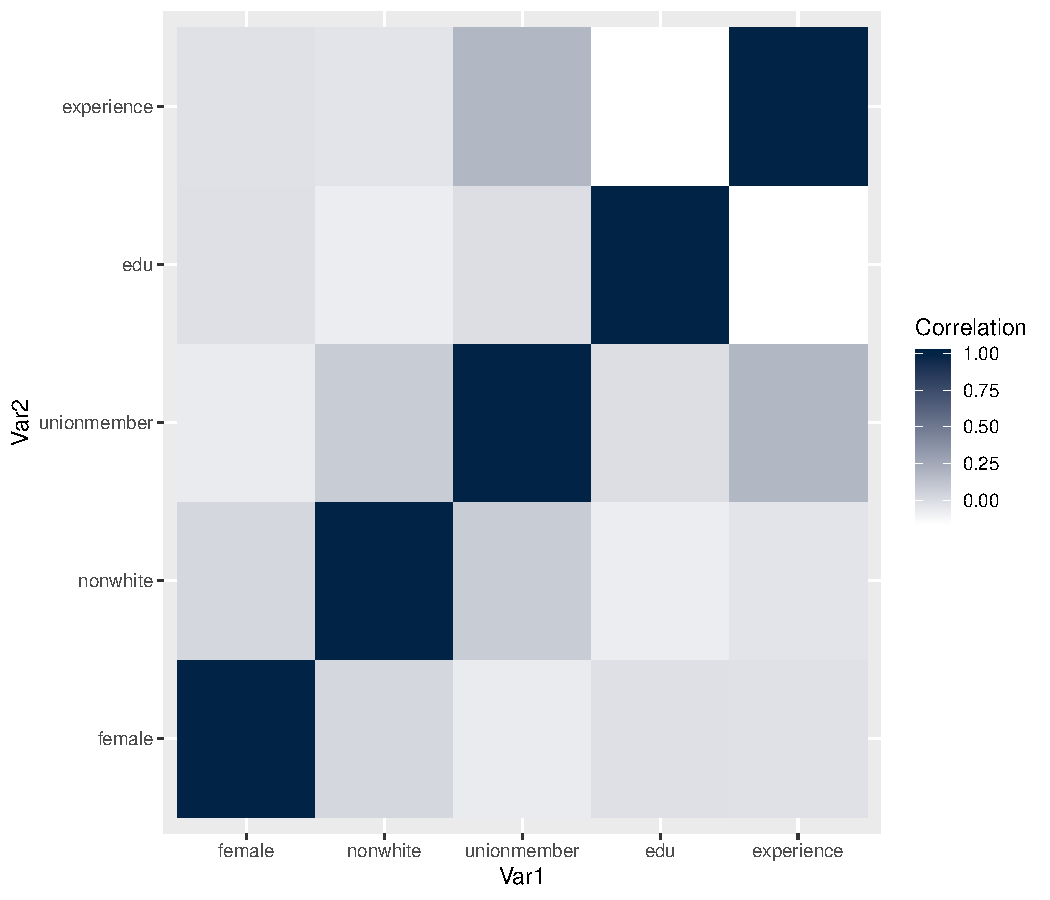
\includegraphics{ps1-Q2-3b}

\item
Run the full regression model and capture your output in a table.

\begin{Schunk}
\begin{Sinput}
R> regressors <- cbind(1, data[, -which(names(data) %in% c("wage"))])
R> colnames(regressors)[1] <- "constant"
R> X <- as.matrix(regressors)
R> k <- ncol(X)
R> n <- nrow(X)
R> y <- data[, "wage"]
R> bols <- solve(t(X) %*% X) %*% (t(X) %*% y)
R> e <- y - X %*% bols
R> SSR <- t(e) %*% e
R> s2 <- (t(e) %*% e) / (n-k)
R> Vb <- s2[1, 1] * solve(t(X) %*% X)
R> se <- sqrt(diag(Vb))
R> t <- bols / se
\end{Sinput}
\end{Schunk}

\begin{Schunk}
\begin{Sinput}
R> df5 <- data.frame(col1=names(regressors),
+                  col2=bols,
+                  col3=se,
+                  col4=t
+                  )
R> colnames(df5) <- c("variable", "estimate", "s.e.", "t")
\end{Sinput}
\end{Schunk}

% latex table generated in R 3.6.2 by xtable 1.8-4 package
% Tue Feb 11 02:13:29 2020
\begin{table}[!h]
\centering
\caption{OLS Estimation - Wage data} 
\begin{tabular}{lrrr}
  \hline
variable & estimate & s.e. & t \\ 
  \hline
constant & -8.5786 & 1.1611 & -7.3884 \\ 
  female & -3.0985 & 0.4237 & -7.3132 \\ 
  nonwhite & -1.6072 & 0.6032 & -2.6644 \\ 
  unionmember & 0.8212 & 0.5832 & 1.4082 \\ 
  edu & 1.4983 & 0.0751 & 19.9483 \\ 
  experience & 0.1697 & 0.0185 & 9.1973 \\ 
   \hline
\end{tabular}
\end{table}

We have calculated $\text{SSR} = $ 44283.640 for this regression analysis. 
\ksp
\item
Re-run the model without ``experience'' (and keep ``age'' out as well).  How do the results change?
What do your findings suggest regarding the correlation of ``experience'' with the remaining regressors?
Is the correlation strong enough to induce noticeable omitted variable bias?

\ksp 

Eliminating "experience" has not impacted most of the covariates considerably, with the exception of "unionmember" which has assumed a biased estimated value of higher magnitude. This suggest the existence of correlation between "unionmember" and the dropped variable "experience", which can align with an interpretation of the relation between the two variables that one may imagine. The correlation however is not dominating to an extent that causes unacceptable omitted variable bias.
\begin{Schunk}
\begin{Sinput}
R> regressors <- cbind(1, data[, -which(names(data) %in% c("wage", "experience"))])
R> colnames(regressors)[1] <- "constant"
R> X <- as.matrix(regressors)
R> k <- ncol(X)
R> n <- nrow(X)
R> y <- data[, "wage"]
R> bols <- solve(t(X) %*% X) %*% (t(X) %*% y)
R> e <- y - X %*% bols
R> SSR <- t(e) %*% e
R> s2 <- (t(e) %*% e) / (n-k)
R> Vb <- s2[1, 1] * solve(t(X) %*% X)
R> se <- sqrt(diag(Vb))
R> t <- bols / se
\end{Sinput}
\end{Schunk}

\begin{Schunk}
\begin{Sinput}
R> df6 <- data.frame(col1=names(regressors),
+                  col2=bols,
+                  col3=se,
+                  col4=t
+                  )
R> colnames(df6) <- c("variable", "estimate", "s.e.", "t")
\end{Sinput}
\end{Schunk}

% latex table generated in R 3.6.2 by xtable 1.8-4 package
% Tue Feb 11 02:13:29 2020
\begin{table}[!h]
\centering
\caption{OLS Estimation - Wage data} 
\begin{tabular}{lrrr}
  \hline
variable & estimate & s.e. & t \\ 
  \hline
constant & -3.8082 & 1.0815 & -3.5211 \\ 
  female & -3.1658 & 0.4411 & -7.1776 \\ 
  nonwhite & -1.9937 & 0.6265 & -3.1821 \\ 
  unionmember & 1.8002 & 0.5970 & 3.0156 \\ 
  edu & 1.3787 & 0.0770 & 17.9003 \\ 
   \hline
\end{tabular}
\end{table}

We have calculated $\text{SSR} = $ 48052.202 for this regression analysis. 

\end{enumerate}

%%%%%%%%%%%%%%%%%%%%%%%%%%%%%%%%%%%%%%%%%%%%%%%%%%%%%%%%%%%%%%%%%%%%%%%%
\section*{Question 3: Orthogonality and Projection}
%%%%%%%%%%%%%%%%%%%%%%%%%%%%%%%%%%%%%%%%%%%%%%%%%%%%%%%%%%%%%%%%%%%%%%%%%%

Consider the ``residual maker matrix'' $\mlt{M}$ and the projection matrix $\mlt{P}$.
Show formally that the following hold (please type all Math in LaTeX):\\

\begin{enumerate}
\item $\kM\kX=\mlt{0}$ (Provide intuition).
\begin{align*}
\kM\kX & = (I - \kX(\kX\kt\kX)^{-1}\kX\kt)\kX \\ & = \kX-\kX(\kX\kt\kX)^{-1}\kX\kt\kX = \kX-\kX=0
\end{align*}

The orthogonality (and hence lack of correlation) between the residual maker $\kM$ and regressors $\kX$ results in transformation of $\ky$ into "everything $\kX$ could not explain"! One way of interpreting this result is that if $\kX$ is regressed on $\kX$, a perfect fit will result and the residuals will be zero.

\item $\kP\kX=\kX$   (Provide intuition).
\begin{align*}
\kP\kX & = \kX(\kX\kt\kX)^{-1}\kX\kt\kX \\ & = \kX \mlt{I} = \kX
\end{align*}

As opposed to the case above, the projection matrix $\kP$ transforms $\ky$ into "everything that $\kX$ is able to explain", that is the fitted values. In other words, $\kX$ is invariant under $\kP$.

\item $ \ky=\kP\ky + \kM*\ky$ (Provide intuition)
\begin{align*}
\kP\ky + \kM*\ky & = \kX(\kX\kt\kX)^{-1}\kX\kt\ky + (\mlt{y}-\kX(\kX\kt\kX)^{-1}\kX\kt)\ky \\ & = \mlt{I}\ky=\ky
\end{align*}
Obviously, $\ky$ can be partitioned into two parts, one that can be explained via $\kX$ and one that can not be explained via the regressors $\kX$. Adding these two parts can "reconstruct" the original $\ky$. In other words, summing up $\kX$ transformed via these two complementary projections gives us the whole information that was to be captured from $\ky$, reversing the decomposition.

\item $\kP\kM=\mlt{0}$
  \begin{align*}
  \kP\kM & = \kX(\kX\kt\kX)^{-1}X\kt(\mlt{I}-\kX(\kX\kt\kX)^{-1}\kX\kt) - \kX(\kX\kt\kX)^{-1}\kX\kt = 0
  \end{align*}

\item $\ke\kt\ke = \ke\kt\ky$
  \begin{align*}
  \ke\kt\ke & = (\kM\ky)\kt(\kM\ky) = \ky\kt\kM\ky = (\kP\ky+\kM\ky)\kt\kM\ky = \ky\kt\kP\kM\ky + \ky\kt\kM\kM\ky \\ & = (\kM\ky)\kt\ky = \ke\kt\ky
  \end{align*}

\item $\ky\kt\ky=\hat{\ky}\kt\hat{\ky}+ \ke\kt\ke$
  \begin{align*}
  \ky\kt\ky & =(\kP\ky + \kM\ky)\kt(\kP\ky + \kM\ky) \\ & = (\kP\ky)\kt(\kP\ky) + (\kP\ky)\kt(\kM\ky) + (\kM\ky)\kt(\kP\ky) + (\kM\ky)\kt(\kM\ky) \\ & = \hat{\ky}\kt\hat{\ky} + \hat{\ky}\kt\kP\kM\ky + \hat{\ky}\kt\kM\kP\ky + \ke\kt\ke \\ & = \hat{\ky}\kt\hat{\ky}+ \ke\kt\ke
  \end{align*}
\end{enumerate}






\begin{Schunk}
\begin{Sinput}
R> proc.time()-tic
\end{Sinput}
\begin{Soutput}
   user  system elapsed 
  0.721   0.089   0.814 
\end{Soutput}
\end{Schunk}

\end{document}        

